\documentclass[conference]{IEEEtran}
\IEEEoverridecommandlockouts
% The preceding line is only needed to identify funding in the first footnote. If that is unneeded, please comment it out.
\usepackage{cite}
\usepackage{svg}
\usepackage{amsmath,amssymb,amsfonts}
\usepackage{algorithmic}
\usepackage{graphicx}
\usepackage{textcomp}
\usepackage{xcolor}
\usepackage{float}
\usepackage{url}
\def\BibTeX{{\rm B\kern-.05em{\sc i\kern-.025em b}\kern-.08em
    T\kern-.1667em\lower.7ex\hbox{E}\kern-.125emX}}
\begin{document}

\title{Applying Soft Actor-Critic to OpenAI Ant\\
}

\author{\IEEEauthorblockN{Zubin Bhuyan}
\IEEEauthorblockA{Student id: 01744486 \\
zubin\_bhuyan@student.uml.edu }
}

\maketitle

\begin{abstract}
In recent years, deep reinforcement learning has been successfully employed to solve a plethora of challenging problems. These RL algorithms are not just limited to simulations, but can be used in robots in real life. One such model-free approach is the Soft Actor Critic algorithm which allows for efficient learning from samples and better stability. This report discusses how SAC can be used for training to adapt with abruptly introduced limitations in robot capability and the robot can make improvements over time. Simulation of SAC was done on the Ant envionment in Open AI Gym framework.\\

\end{abstract}

\begin{IEEEkeywords}
reinforcement learning, soft actor critic, openai
\end{IEEEkeywords}

\section{Introduction}
\emph{Reinforcement Learning} is a form of machine learning where an agent ``learns" from its experiences and strives to maximize its rewards by choosing the most appropriate action. It has been the area of interest for researchers from a vast number of domains, especially because the reward-driven approach is suitable for a many problems requiring an exploratory approach to a solution.

Advances in the last decade has enabled reinforcement learning approaches to take advantage of deep neural architectures (Fig \ref{figDeepRL}\footnote{Image source: \url{http://bit.ly/2WcqoIn}} ). RL approaches have been successfully applied not only to simulations\cite{mnih2015humanlevel}, but to real world tasks\cite{DBLP:journals/corr/abs-1812-00568} as well. 

\begin{figure}[htbp]
\centerline{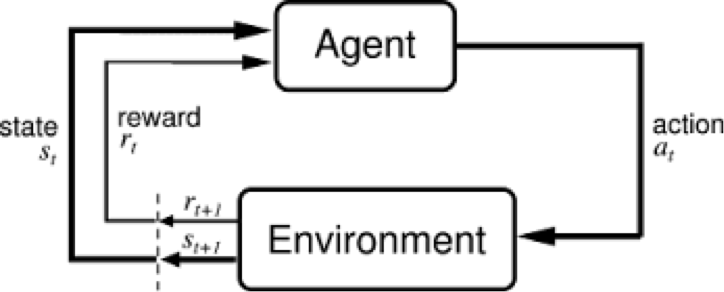
\includegraphics[scale=0.5]{img/simple_RL_schema.png}}
\caption{A simple RL schema.}
\label{figRL}
\end{figure}
Traditional reinforcement learning paradigm comprise of an \textit{environment} and an \textit{agent}. The agent can perform a set of \textit{actions} which takes it from one \textit{state} to another, and with each transition is associated a \textit{reward}. Fig \ref{figRL} is a simple representation of the RL schema. The goal is to maximize the rewards collected over time. Policy is the term used to describe the rule based on which an agent takes actions. Policies in deep RL are parameterized, and these parameters are tweaked to achieve the most optimal policy possible.

Two approaches of model-free RL are \textit{policy optimization} (learning an approximator value function) and \textit{Q-learning}, which requires learning an approximate $Q_{\theta}(s,a)$. A more detailed explanation of RL concepts and ideas can be found in \cite{Sutton:1998:IRL:551283}.

While there can be many variations in the low-level implementation, this is the high-level idea of reinforcement learning usually remains the same. Fig \ref{figRLFam} is a non-exhaustive RL algorithm classification \footnote{Image source: \url{https://bit.ly/30b3zb3}}.


The focus of this report will be on Soft Actor Critic (SAC) algorithm \cite{DBLP:journals/corr/abs-1801-01290} which has been shown to be able to applicable to a number of real life situations\cite{refSACapplication}. 

\begin{figure}[htbp]
\centerline{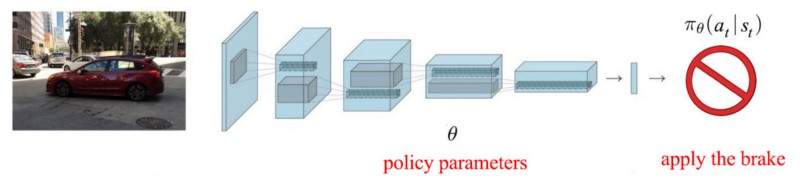
\includegraphics[width=\linewidth]{img/imgDeepRL.jpg}}
\caption{A general representation of how deep NN architecture is used for RL.}
\label{figDeepRL}
\end{figure}

The subsequent section discusses some previous work done in this area. Section \ref{secMethod} describes the methodology of SAC. This is followed by section \ref{secExp} which describes the experimental setup and the results. Section \ref{secConclusion} is the conclusion.


\begin{figure}[htbp]
  \centering
  \centerline{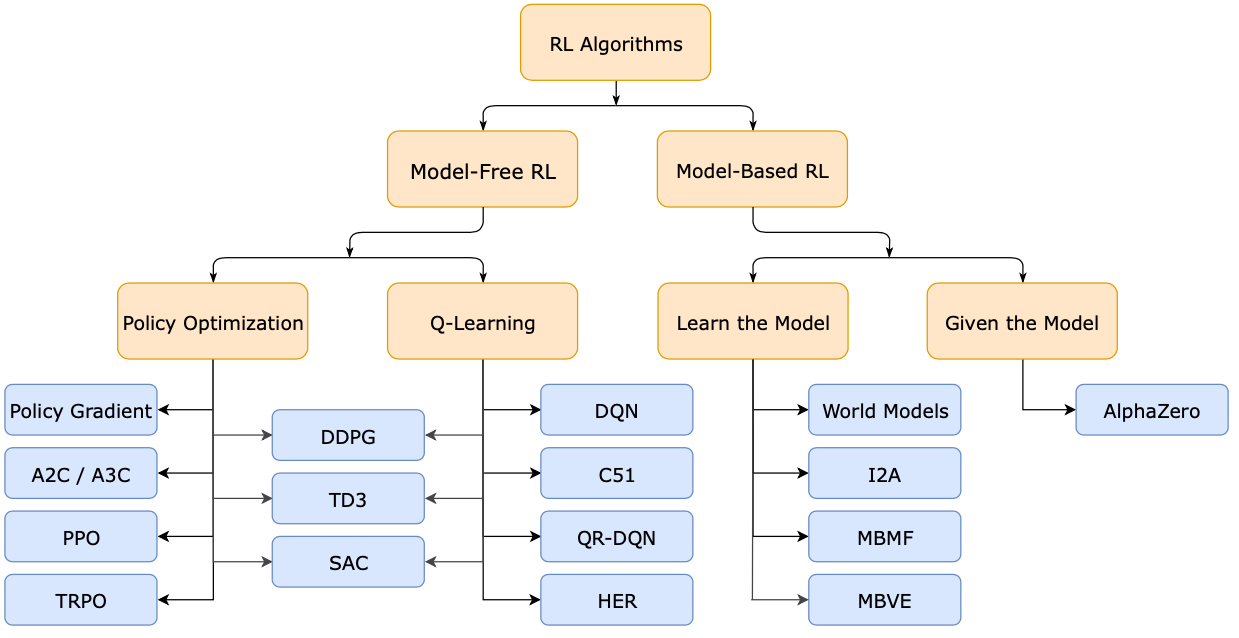
\includegraphics[width=\linewidth]{img/figRL-fam.png}}
  \caption{Classification of RL algorithms.}
  \label{figRLFam}
\end{figure}

\section{Related Work}\label{secRelated}
Model-free policy optimization Advantage Actor Critic algorithms perform gradient ascent directly to maximize the reward. In such methods the \textit{critic} estimates a value function (either of $Q$ or $V$), and the policy is updated by the \textit{actor}. Both the functions of \textit{actor} and \textit{critic} are parameterized with deep neural networks, which are updated in every step of training.

Asynchronous Advantage Actor Critic (A3C) \cite{DBLP:journals/corr/MnihBMGLHSK16} is an actor-critic method where multiple workers perform parallel training and independeltly update a global value function. The independent nature of the workers allow for a more effective exploration. The A3C architecture is illustrated in fig \ref{figA3C}.

\begin{figure}[htbp]
  \centering
  \centerline{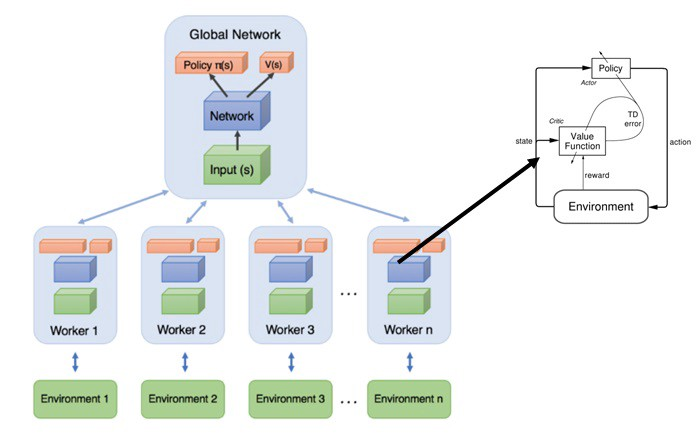
\includegraphics[width=\linewidth]{img/imgA3C.jpeg}}
  \caption{Architecture of A3C.}
  \label{figA3C}
\end{figure}

The idea of maximizing entropy for learning adaptive behaviour was explored in \cite{ziebart2010modelingB} and \cite{ziebart2008maximum}. It has been shown that policies maximizing entropy led to more exhaustive exploration and better action sequences \cite{DBLP:journals/corr/HaarnojaTAL17}. 

\section{Methodology}\label{secMethod}
Soft-Actor critic (SAC) \cite{DBLP:journals/corr/abs-1801-01290} is a model-free, off-policy RL method which is relatively more sample efficient than other algorithms. Another advantage of SAC is that it is ``robust to brittleness in convergence" or adaptive to a changing environment. The main idea of SAC is \textit{entropy regularization}, i.e. it seeks to maximize the policy entropy so that it encourages more exploration. This results in a higher likelihood of actions with similar Q\-values getting same probability. The following SAC objective function comprises of an additional entropy term along with the usual reward term. 
\begin{figure}[H]
\centering
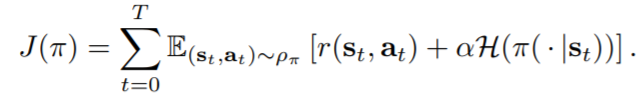
\includegraphics[width=\linewidth]{img/figSACeq1.png}
\end{figure}
A Q-network is trained with examples with the goal of minimizing the following error
\begin{figure}[H]
\centering
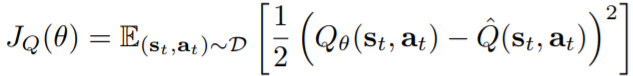
\includegraphics[width=\linewidth]{img/figQNetErr.png}
\end{figure}
A \textit{policy network} is also optimized for parameters. The algorithm is given below:
\begin{figure}[H]
\centering
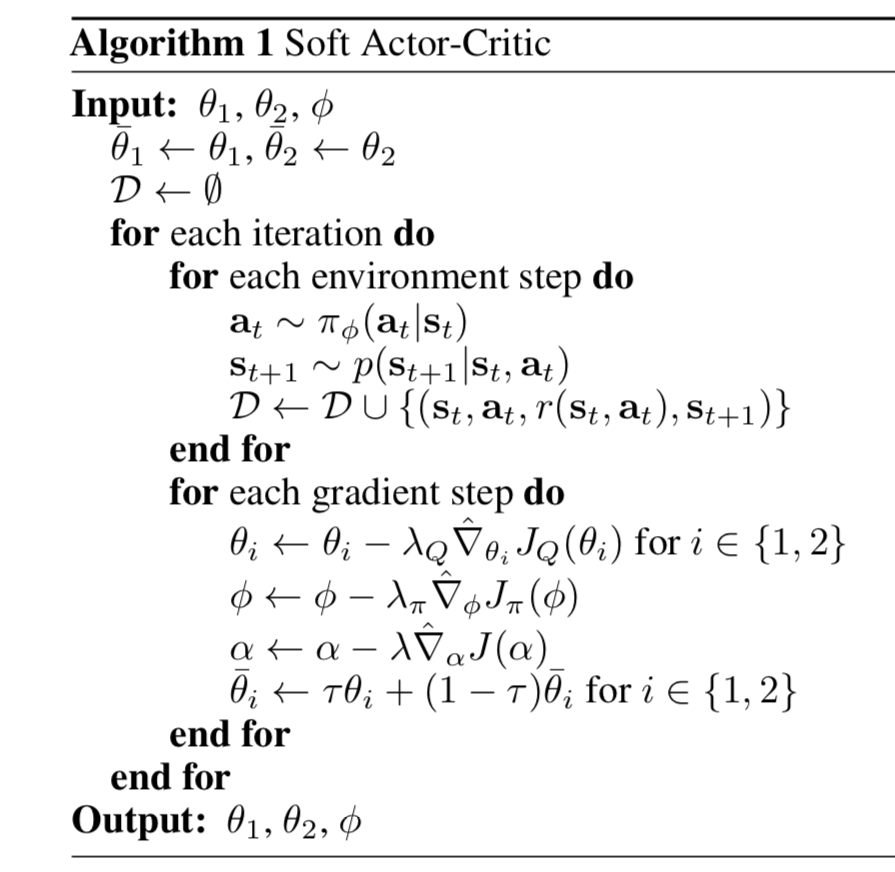
\includegraphics[width=\linewidth]{img/figSACAlgo.png}
\end{figure}

This algorithm has been tested on the Minitaur robot (for a walking task on unknown terrain), and the Dynamixel Claw (valve rotation task).

In this project we use the SAC algorithm to train the Ant agent of OpenAI Gym to walk in regular condition and compare the results when one of its legs is disabled. The experiments are described in details in the next section.

\section{Experiments and Results}\label{secExp}
\subsection{Experimental setup}
The primary goal of the experiments were to evaluate if the four-legged Ant\cite{AntEnv}, learning to walk with the soft-actor algorithm, could cope with the adversity of losing one of its limbs. The OpenAI Gym \cite{openAIgym} toolkit was used along with the MuJoCo\cite{todorov2012mujoco} Ant environment. \textit{rlkit}\footnote{\url{https://github.com/vitchyr/rlkit}}, a Python repository of reinforcement learning algorithms, was used for initial testing. Two other repositories\footnote{\url{https://github.com/haarnoja/sac}} \footnote{\url{https://github.com/vitchyr/rlkit}} were also used for reference.

All simulations were performed on Virtual Machines on Google Cloud platform. These VMs each had $8$ vCPUs, $30$ GB of memory, $80$ GB of SSD and one NVIDIA $K80$ graphcs card.

\subsection{Simulation parameters and hyperparameters}
The simulations for which the graphs are given below, a \emph{learning rate} of $0.003$, \emph{temperature} value of $0.1$, a \emph{replay buffer} of $100,000$, and a \emph{discount factor} of $0.99$. Batch size for training was $256$, optimizer used was \emph{Adam}, activation function was ReLU, and policy was evaluated every $10$ episodes.

The VMs were accessable through a console interface; the results of the simulations were stored as Tensorboard logs and were viewed later on a laptop.

\subsection{Results}
\subsubsection{Training Ant with 4 legs}
The reward achieved while testing and training were logged with the Tensorboard module. Fig \ref{fig4legtrain} and \ref{fig4legtest} show how the reward values. for training and testing gradually increase with increasing episodes. This training was done for 1350 episodes, which took about than 9 hours to complete.


\begin{figure}[htbp]
\centerline{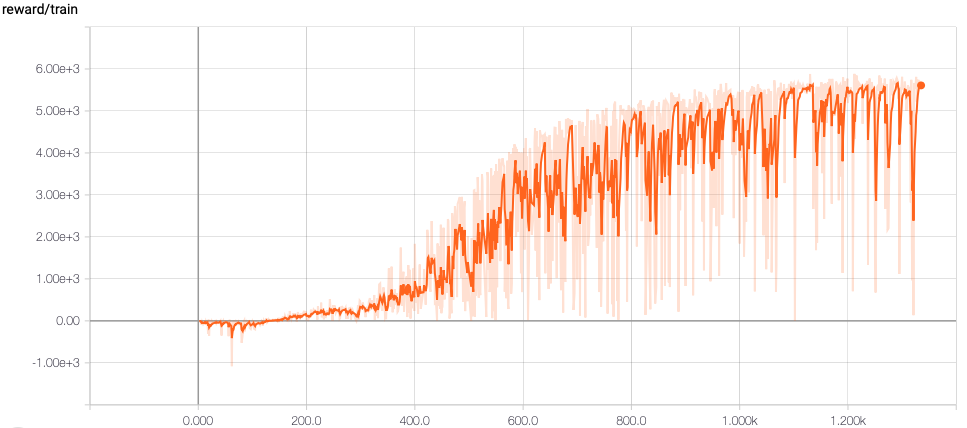
\includegraphics[width=\linewidth]{img/ant4-reward-train.png}}
\caption{Reward curve for training the Ant with 4 legs.}
\label{fig4legtrain}
\end{figure}

\begin{figure}[htbp]
\centerline{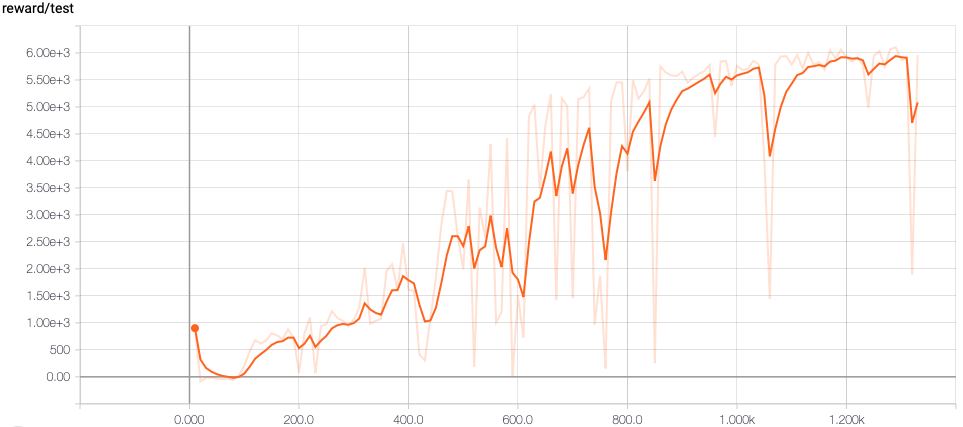
\includegraphics[width=\linewidth]{img/ant4-reward-test.png}}
\caption{Reward curve while testing the Ant environment with 4 legs.}
\label{fig4legtest}
\end{figure}

\subsubsection{Disabling one leg after 700 episodes of training}
For the second part of the experiment, the agent was required to walk with 3 legs. So, after initial training of 700 episodes with 4 legs, one leg was disabled. The initial training was given so that the agent would at least get a change for some free exploration.
Fig \ref{fig4legtest} and \ref{fig1legdisabledtest} show how the rewards change over time as the training goes on. We can observe that there is a steep fall in the reward after a leg is disabled. However, the value quickly goes up again, indicating that the agent was somehow able to move even with three legs. It should also be noted here that the rewards are not as high as it was with 4 legs. 

A simulation was also done where one leg is disabled and agent gets no prior training. The reward values obtained in testing this case for 625 episodes of training is shown in fig \ref{fig3legnotrain}. The graph indicates that the agent struggles to perform the task, where as in the other cases the agent's reward was increasing at 625 episode. 

\begin{figure}[htbp]
\centerline{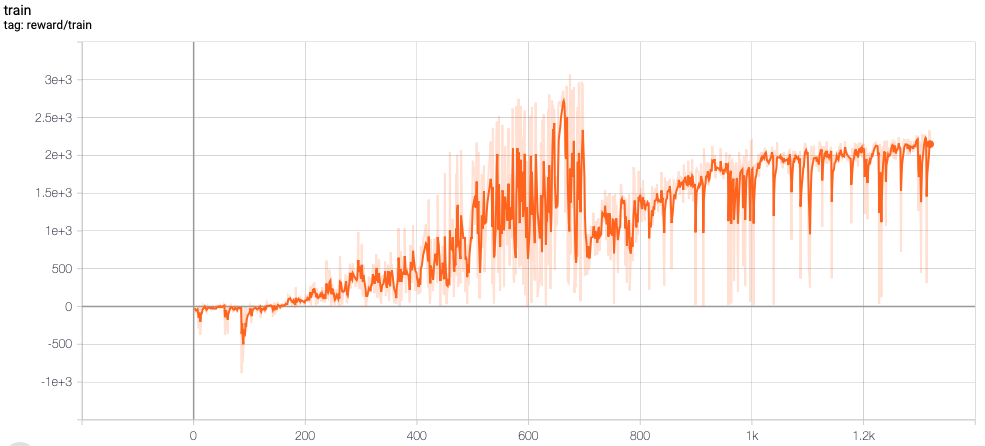
\includegraphics[width=\linewidth]{img/ant-1-disabled-reward_train.png}}
\caption{Training the Ant agent with 3 legs (with initial 4-legged training of 700 episodes).}
\label{fig1legdisabledtrain}
\end{figure}

\begin{figure}[htbp]
\centerline{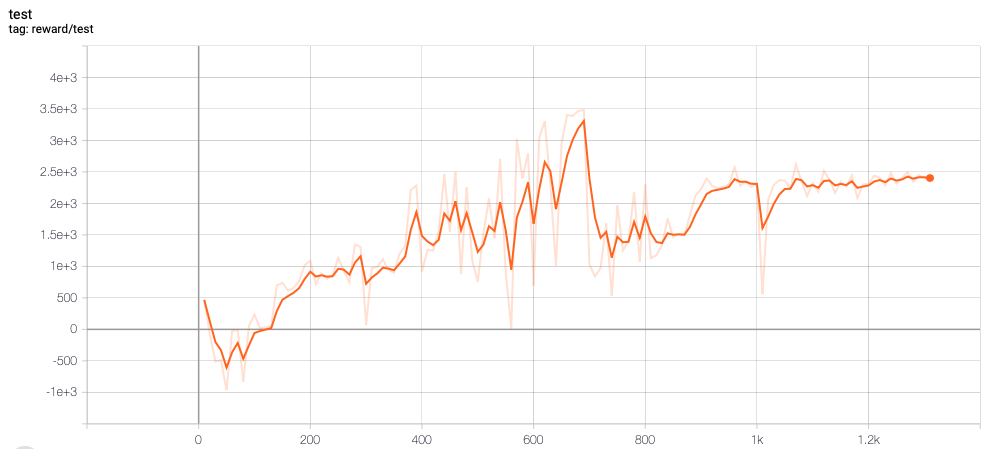
\includegraphics[width=\linewidth]{img/ant-1-disabled-reward_test.png}}
\caption{Testing the Ant agent with 3 legs after every 10 epochs (with initial 4-legged training of 700 episodes).}
\label{fig1legdisabledtest}
\end{figure}

\begin{figure}[htbp]
\centerline{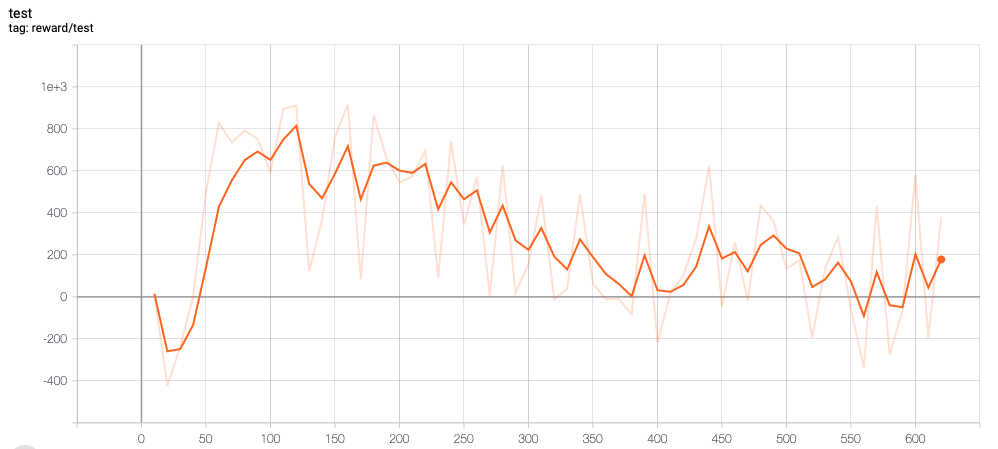
\includegraphics[width=\linewidth]{img/ant-3leg-no4.png}}
\caption{Reward graph for agent with 1 leg disabled (no prior training).}
\label{fig3legnotrain}
\end{figure}

\begin{figure}[htbp]
\centerline{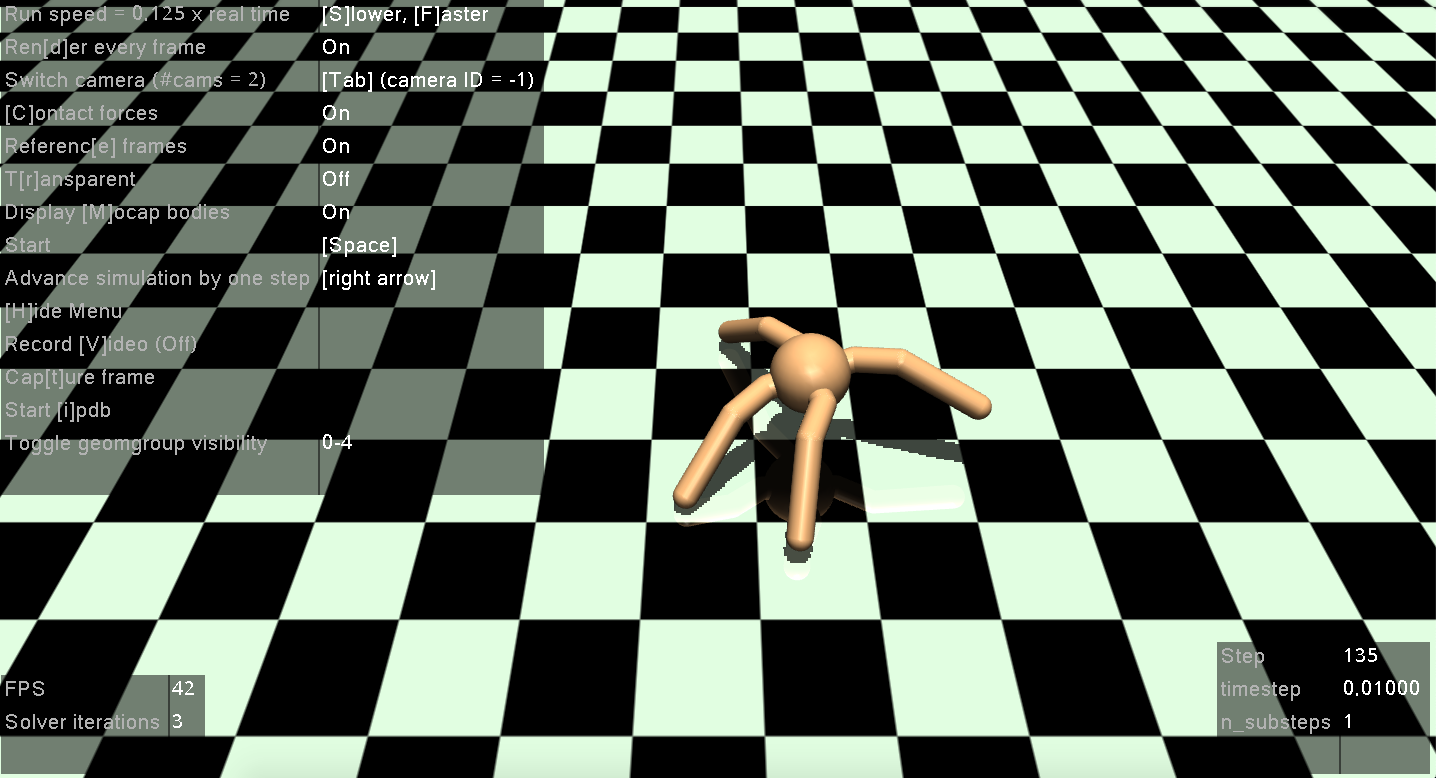
\includegraphics[width=\linewidth]{img/imgAntVis.png}}
\caption{Visualizing trained Ant agent with 4 legs.}
\label{fig3legnotrain}
\end{figure}

\section{Conclusion}\label{secConclusion}
This report presents a study of application of soft actor critic algorithm to the four-legged Ant agent in OpenAI Gym. Simulations were performed for different cases where one of the legs would be arbitrarily disabled. It was observed that if the agent had some training with 4 legs before one of its legs was turned off, it could adapt faster than than the case where it had no prior training.

This work can be further extended to analyze how much of prior training can be considered to be sufficient in order for an agent to complete a task with limited capabilities or in adversarial conditions. There is also scope for improvement in exploration during training for situations where initial training is not available.
\\

\bibliographystyle{ieeetr}
\bibliography{ref}
\vspace{12pt}

\end{document}
